%\documentclass{hitec}
\documentclass{myhitec}
\usepackage[UTF8]{ctex}
\usepackage{fontspec}
\usepackage[dvipsnames]{xcolor}
\usepackage{amsmath}
\usepackage{array}
\usepackage{graphicx}
\usepackage{longtable}
\usepackage{booktabs}  %用于美观表格线宽
\usepackage{multirow}  %用于跨行表
\usepackage{tabularx}  %定义表格宽度
\usepackage{float}
\usepackage{indentfirst}
\usepackage{bibentry}
%\usepackage[linkcolor=gray!40!black]{hyperref}
\usepackage[colorlinks,urlcolor=blue!50!black,linkcolor=blue!50!black,anchorcolor=blue,citecolor=blue!50!black,CJKbookmarks=True]{hyperref}
\usepackage{tcolorbox}
\usepackage{hyperref} % This line is readily ommited of it makes trouble
\tcbuselibrary{breakable,listings,skins,fitting}
\usepackage{newenviron}

%\usepackage{changepage}
%\begin{adjustwidth}{2cm}{1cm}
%\end{adjustwidth}

%==========================================
% Latex 命令环境设置
%==========================================

%==========================================
% 字体设置
%==========================================
%\newfontfamily{\monoca}{Monaco}
\newfontfamily{\monoca}{Microsoft YaHei}
% \setCJKmainfont{FandolSong}
% \setmainfont{FiraSans-Light}
% \setsansfont{FiraSans-Hair}
% \setmonofont{FiraMono-Regular}

\setCJKmainfont{Microsoft YaHei}
% \setmainfont{Microsoft YaHei}
% \setsansfont{Microsoft YaHei}
% \setmonofont{Microsoft YaHei}

\setmainfont{Consolas}
\setsansfont{Consolas}
\setmonofont{Consolas}


%==========================================
% 自定义命令设置
%==========================================
\newcommand{\urllink}[2]{\href{#1}{#2}}

\newcommand{\HT}{\textsc{\raisebox{0.1em}{H}\raisebox{-0.1em}{I}%
	\raisebox{0.1em}{T}\raisebox{-0.1em}{E}\raisebox{0.1em}{C} }}

\newtheorem{thm}{定理}
\newcommand\degree{^\circ}

\newtcbox{\emphasizebox}[1][blue]{enhanced,on line,%drop fuzzy shadow,
arc=2pt,outer arc=2pt,colback=#1!5!white,colframe=#1!50!black,
boxsep=0pt,left=3pt,right=3pt,top=1pt,bottom=1pt,
colupper=blue!50!black,fit basedim=10pt,
boxrule=0.1pt,bottomrule=0.1pt,toprule=0.1pt,nobeforeafter}

%==========================================
% 自定义lsting设置
%==========================================
\newtcblisting{messagebox}{%
breakable,
left=3mm,
listing only,
boxrule=0.2mm,
colback=gray!5,
fontupper=\monoca,colupper=red!50!black,
coltext=black
}%

\newtcblisting{commandbox}{%
breakable,
left=3mm,
listing only,
boxrule=0.2mm,
colback=black,
fontupper=\monoca,colupper=red!50!black,
coltext=green
}%

\newtcblisting{codeout}{%
breakable,
left=3mm,
boxrule=0.2mm,
colback=gray!5,
fontupper=\monoca,colupper=red!50!black,
coltext=black
}%

%\lstset{
    % numbers=left,
    % %numberstyle={\color{lightgray}},
    % numberstyle={\color{green}},
    % backgroundcolor={\color[RGB]{41, 47, 51}}, %背景颜色
    % basicstyle={\color[RGB]{208, 214, 219}}, %普通字符串颜色
    % stringstyle={\color[RGB]{0, 128, 0}}, %字符串颜色
    % keywordstyle={\color[RGB]{101, 140, 230}}, %关键词颜色
    % commentstyle={\color{gray}}, %注释颜色
    % frame=none, %无边框
    % breaklines=true, %自动分行
    % language={[ANSI]C},
    % captionpos=b,
% }

\lstnewenvironment{myccode}[1][]
{\lstset{
    numbers=left,
    %numberstyle={\color{lightgray}},
    %frame=none, %无边框
    frame=lines, %上下线
    %frame=single, %边框
    language={[ANSI]C},
    breaklines=true, %自动分行
    %keywordstyle={\color{blue}}, %关键词颜色
    %stringstyle={\color{orange}}, %字符串颜色
    %stringstyle={\color{magenta}}, %字符串颜色
    %commentstyle={\color{green}}, %注释颜色
    %basicstyle={\color[black]}, %普通字符串颜色
    %captionpos=b,
    #1
        }
}
{}

%==========================================
% 标签格式
%==========================================
\hypersetup{
    colorlinks=true,
    bookmarksnumbered=true,
    pdftitle={My LaTeX2e note},
    pdfkeywords={LaTex, note},
}

%==========================================
% 摘抄格式
%==========================================
\newenvironment{literbox}
%{\begin{messagebox}
{\begin{quote}\zihao{-4}\kaishu
%{\zihao{-3}\kaishu
}
%{\end{messagebox}}
{\end{quote}}
%{}

%==========================================
% 图片路径
%==========================================
\graphicspath{{figure/}, 
{005_protocol_note/bt_picture/}, 
{009_soft_install_note/gvim_install_picture/}, 
{008_system_work_note/system_note_picture/}, 
}

%==========================================
% 水印
%==========================================
%\usepackage{draftwatermark}
%\SetWatermarkText{Zero Note} % the Text
%\SetWatermarkLightness{0.9} % the lightness from 0 to 1, default 0.8
%\SetWatermarkScale{1.0} % the scale, default 1.2


%==========================================
% 首页信息
%==========================================
\title{工作笔记}
\author{莫志烨}
\company{纯属个人}
\confidential{\textbf{-- 非限制发布 --}}

%==========================================
% 开始排版
%==========================================
\begin{document}
\begin{titlepage}
\maketitle
这是一篇关于\LaTeX 的文档,风格使用 \HT 。
\end{titlepage}

%\begin{abstract}
%本文说明如何用\LaTeX{}模板撰写报告。
%
%\end{abstract}
%提示:获取本文档的最新版本比现在开始阅读更重要。
%本文的最新版本见于:\url{https://git.coding.net/yangdawei/git.git}
\tableofcontents
\newpage
\newpage

%==========================================
% 图片路径
%==========================================
\graphicspath{{figure/},
{002_latex_note/picture/},
{005_protocol_note/bt_picture/},
{009_soft_install_note/gvim_install_picture/},
{008_system_work_note/system_note_picture/},
}

%==========================================
% 章节内容
%==========================================
\section{\LaTeX 应用笔记}
本文档于\today 开始使用\LaTeX 作笔记文档。

\subsection{超链接应用}
超链接显示有2种:
\begin{itemize}
\item 链接和显示内容一致:\url{https://www.baidu.com}
\item 链接和显示内容不一致:\href{https://www.baidu.com}{百度链接}
\end{itemize}

\subsection{枚举项应用}
以下是枚举内容:
\begin{itemize}
\item 枚举1。
\item 枚举2。
\item 枚举3。
\item 枚举4。
\end{itemize}


\subsection{在正文中强调某个词语}
我要\emphasizebox{强abc调}这个词语。

\subsection{插入Linux命令}
\begin{commandbox}
 > sudo chsh -s zsh
\end{commandbox}

\subsection{用数字表示一个范围}
我要表示一个范围:$18\sim22$ 岁。

\subsection{插入一个Linux信息输出框}
\begin{messagebox}
On branch master
Your branch is ahead of 'origin/master' by 3 commits.
  (use "git push" to publish your local commits)
Changes not staged for commit:
  (use "git add <file>..." to update what will be committed)
  (use "git checkout -- <file>..." to discard changes in working directory)
\end{messagebox}

\subsection{测试codeout}
\begin{codeout}
codeout ccc
\end{codeout}


\subsection{基本代码块测试}
\begin{lstlisting}[language=C, numbers=left]
void main ()
{
    return;
}
\end{lstlisting}

\subsection{测试mycode}
\begin{myccode}
/* 这是一个hello工程 */
void main ()
{
    int cnt = 0;
    printf("Hello World: %d\n", cnt);
    return;
}
\end{myccode}

\subsection{空行分段 单个换行相当于空格}
老话说生活有五味,酸甜苦辣咸。苦是生命所不能避免的一味,叔本华说:“人生就是痛苦,我们可以把痛苦转换成幸福”,努力就是转化的过程,尽管在这个过程中,我们可能会感到更加辛苦。

苦,是人生的必经过程。人生就是一个“享受”痛苦和磨难的过程,这个过程是值得体会和拥有的。
人生本身就是一场与痛苦并存的旅行,并不像很多人想象的那么轻松,从生下来的那一天,我们就开始了人生的修行。

无论你生长在怎样的环
境中,你都会面临人生的各种难题。面对这些难题、困境,没有人可以不流泪流汗就轻轻松松地跨过去。经历得越多,越容易发现这个世界的真理——越怕吃苦,越有苦吃。那些心灵真正富足的人,其实都不怕吃苦。

\subsection{脚注命令}
苦\footnote{\emph 苦,是人生的必经过程。}

\subsection{引用}
\begin{quote}
老话说生活有五味,酸甜苦辣咸。
\end{quote}

\subsection{改变字体和字号}
\begin{quote}
\zihao{-5} \kaishu 老话说生活有五味,酸甜苦辣咸。
\end{quote}

\subsection{定理环境}
\begin{thm}[勾股定理]
一二三。
\end{thm}

\subsection{公式排版}
\begin{equation}
a(b+c) = ab + ac
\end{equation}

\begin{equation}
\angle ABC = \pi / 2
\end{equation}

\begin{equation}\label{eq:gougu}
AB^2 = BC^2 + AC^2
\end{equation}

\begin{equation}
90^\circ
\end{equation}

\subsection{插入图片}
%\begin{figure}[ht]
\begin{figure}[H]
\centering
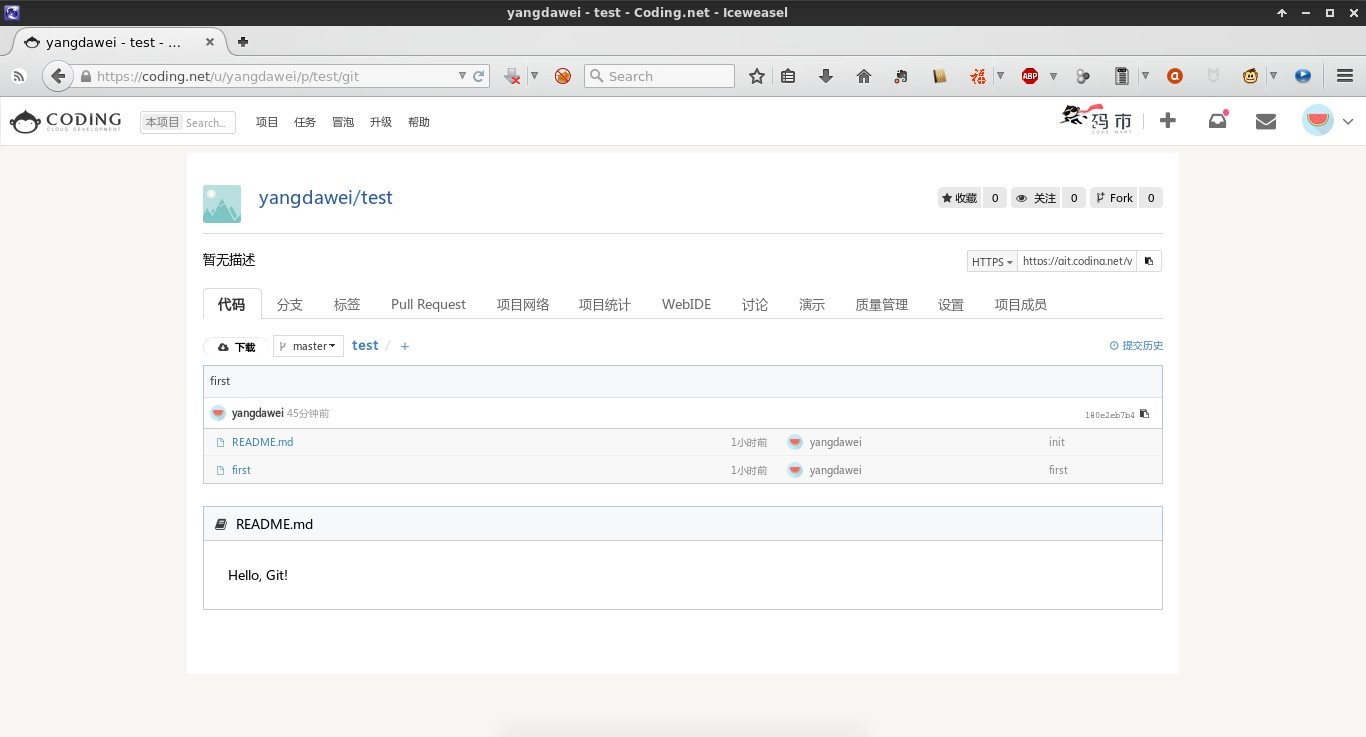
\includegraphics[height=5cm]{testcode.jpg}
\caption{建立项目}
\label{fig:createproject}
\end{figure}

\subsection{插入表格}
\begin{table}[H] %浮动环境
\begin{tabular}{|rrr|}
\hline
直角边 $a$ & 直角边 $b$ & 斜边 $c$ \\
\hline
3 & 4 & 5 \\  %分列
5 & 12 & 13 \\ %下一行
\hline
\end{tabular}
\end{table}

\subsection{引用公式和图表}
图 \ref{fig:createproject} 表示。

公式 \ref{eq:gougu} 方法。

另一种引用公式 \eqref{eq:gougu} 方法。 %添加\usepackage{amsmath}

\subsection{自定义新的命令}
使用newcommand命令。
符号度的新命令 $90\degree$ 。%注意:要加$$

\subsection{一些标点符号}
省略号\ldots \dots \# \quad \$ \quad \% \quad \& \quad \{ \quad \} \quad \_ \quad \textbackslash

中文标点使用全角输入,破折号shift+- ——,省略号shift+6……

忽略每行前面的空格,后面的空格多个当成一个,\TeX\ ing,\TeX{} ing. {\TeX} ing. 换行当空格I 
am Tex.汉字和字母自动添加空格tex。



\section{GIT学习笔记}
\subsection{合并两个提交历史}
连续在本地有两个提交, 如果需要合并这两个提交历史, 使用命令:
\begin{cmd}
 > git rebase -i HEAD~2
\end{cmd}



\section{VIM学习笔记}

\section{通信协议学习笔记}
\subsection{IIC通信协议}

\subsection{UART通信协议}

\subsection{SPI通信协议}

\subsection{IIS通信协议}
\subsubsection{IIS概述}
I2S = Inter-IC Sound = Integrated Interchip Sound = IIS,是飞利浦在1986年定义(1996年修订)的数字音频传输标准,用于数字音频数据在系统内器件之间传输,例如编解码器CODEC、DSP、数字输入/输出接口、ADC、DAC和数字滤波器等。其与IIC无关联。

\subsubsection{IIS硬件结构}
IIS是个相对来说简单的接口协议,没有地址和片选机制。在总线上,只能同时存在一个主设备和发射设备;提供时钟的设备为主设备,可以是发射设备也可以是接收设备,或者是协调两者的其他控制设备。在高端应用场合中,CODEX经常作为主设备以便精确控制IIS的数据流。

%=============================================================%
%                       插入一张图片                          %
%=============================================================%
\begin{figure}[H]
\centering
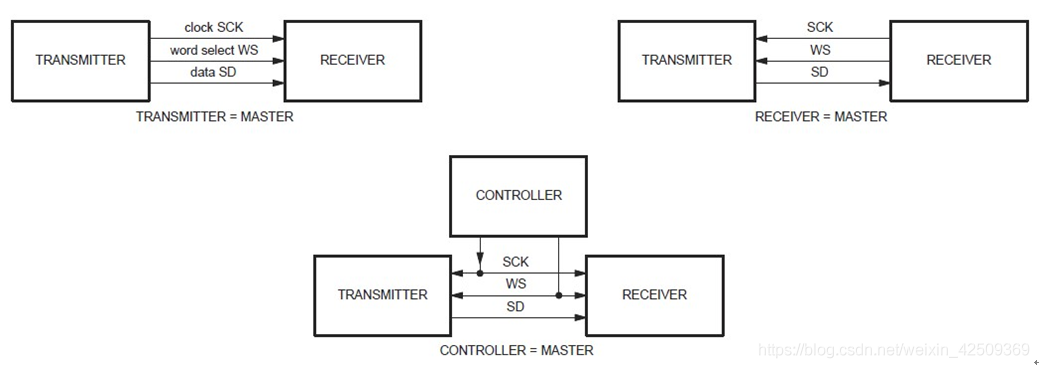
\includegraphics[scale=0.3]{iis_topo.png}
\caption{IIS硬件TOPO结构}
\end{figure}

IIS协议定义三根信号线:时钟信号SCK、数据信号SD和左右声道选择信号WS。
\begin{itemize}
\item WS:声道选择信号,表明数据发送端所选择的声道: WS=0,表示选择左声道,WS=1,表示选择右声道,同时也叫帧时钟,等于声音的采样率。
\item SCK:模块内的同步信号,从模式时由外部提供,主模式时由内部产生。
\item SD:串行数据,以二进制补码形式在数据线上传输;在WS变化后的第一个SCK脉冲,先传输最高位(MSB, Most Significant Bit)。
\end{itemize}

\subsubsection{IIS工作模式}
IIS的操作模式分为三种:标准IIS模式、左对齐模式和右对齐模式。
\begin{itemize}
\item 标准IIS模式(Phillips Standard)

IIS模式是标准左对齐格式再延迟一个时钟位变化来的,时序如下所示:
\begin{figure}[H]
\centering
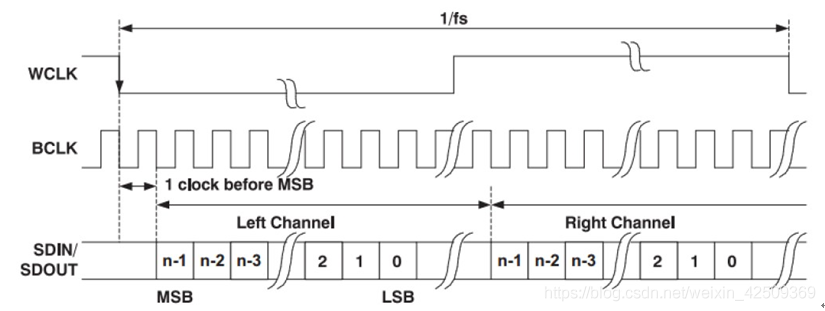
\includegraphics[scale=0.4]{iis_starndar_mode.png}
\caption{标准IIS模式}
\end{figure}
左右通道的数据MSB均是在WS变化后第二个SCK/BCLK上升沿有效。

\item 左对齐模式(Left Justified Standard)

标准左对齐格式的数据的MSB没有相对于BCLK延迟一个时钟。左对齐格式的左右声道数据的MSB在WS边沿变化后SCK/BCLK的第一个上升沿有效。具体如下图所示:
\begin{figure}[H]
\centering
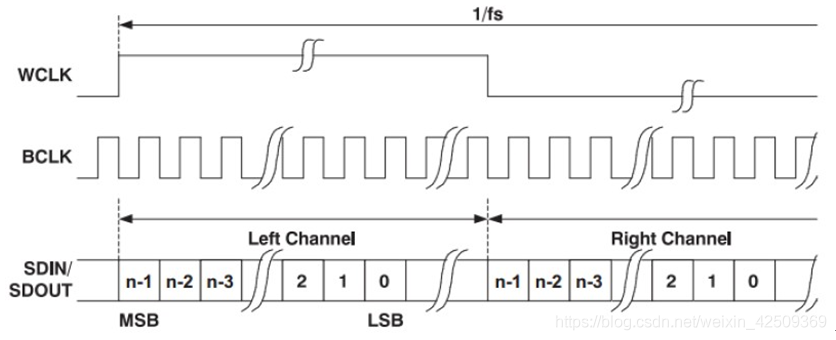
\includegraphics[scale=0.4]{iis_left_mode.png}
\caption{IIS左对齐模式}
\end{figure}
支持16~32bit字长格式;

\item 右边对齐模式(Right Justified Standard)

也叫日本格式,sony格式,具体对齐方式如下图所示:
\begin{figure}[H]
\centering
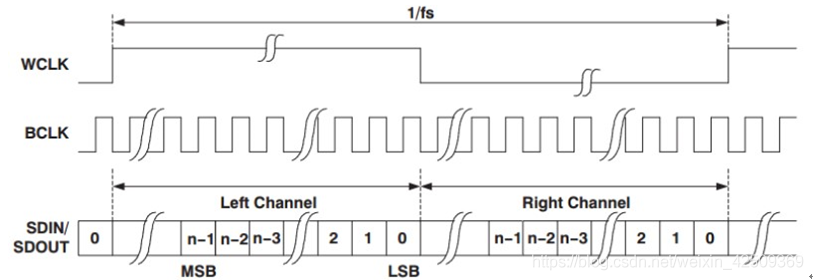
\includegraphics[scale=0.4]{iis_right_mode.png}
\caption{IIS右对齐模式}
\end{figure}
接收设备必须事先知道待传数据的字长。

\end{itemize}

\begin{messagebox}
注意左右对齐模式的WS时钟高电平为左声道,低电平为右声道,刚好与标准IIS相反。
\end{messagebox}

\subsubsection{IIS时钟频率计算}
SCK = 采样率(48K、44.1K、16K等) x  字长(16bit、24bit、32bit) x 2(左右两通道);MCLK/SCK =  384 、256 等需要参考手册说明支持哪种;

\subsubsection{一些问题解答}
\begin{itemize}
    \item \emphasizebox{384, 512fs}代表什么意思?\newline
        256fs中“fs” 就是表示audio sampling frequency, 表示在一个LR周期中BCLK的个数,比如;数据是32bit位宽,2个通道,那么fs就是32 x 2 = 64fs,可以理解为一帧有多少个sclk, fs参数结合采样率(LRCLK)可以算出BCLK,BCLK与MCLK存在分频关系,这个关系与实际通信芯片有关;
\end{itemize}

\subsection{蓝牙通信协议}
\begin{figure}[H]
\centering
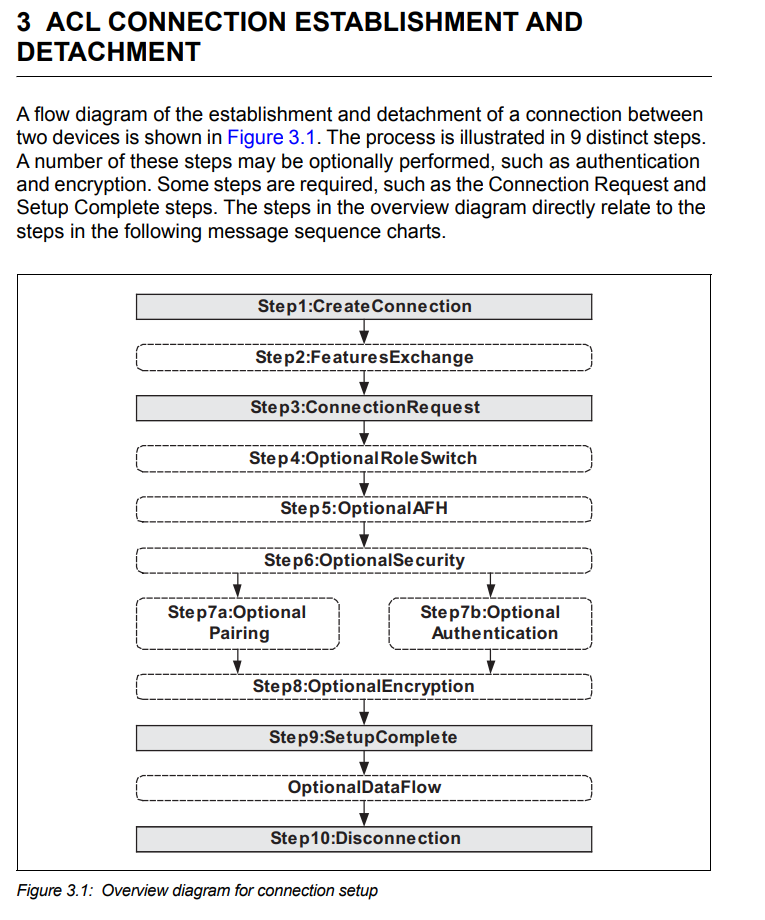
\includegraphics[height=8cm]{connection.png}
\caption{连接步骤}
\label{fig:connection}
\end{figure}

\begin{figure}[H]
\centering
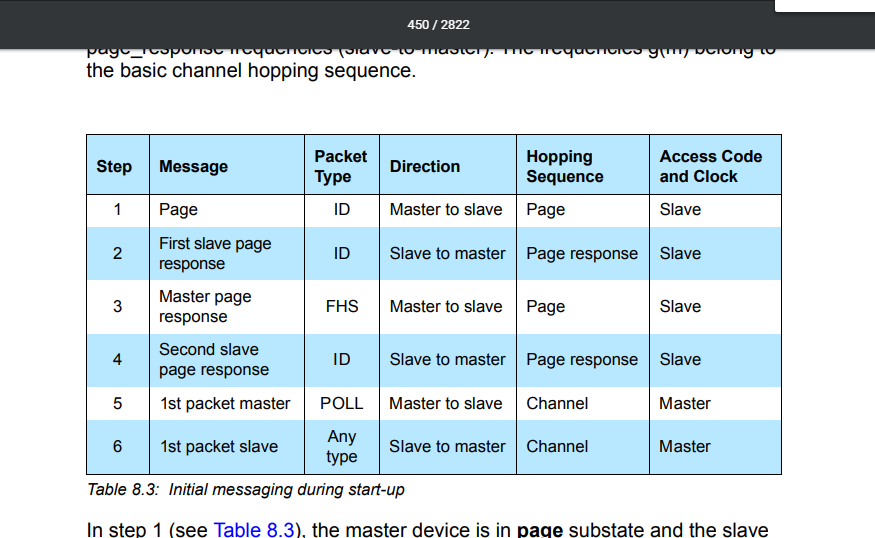
\includegraphics[height=8cm]{page_startup.png}
\caption{pagestartup}
\label{fig:pagestartup}
\end{figure}

\begin{figure}[H]
\centering
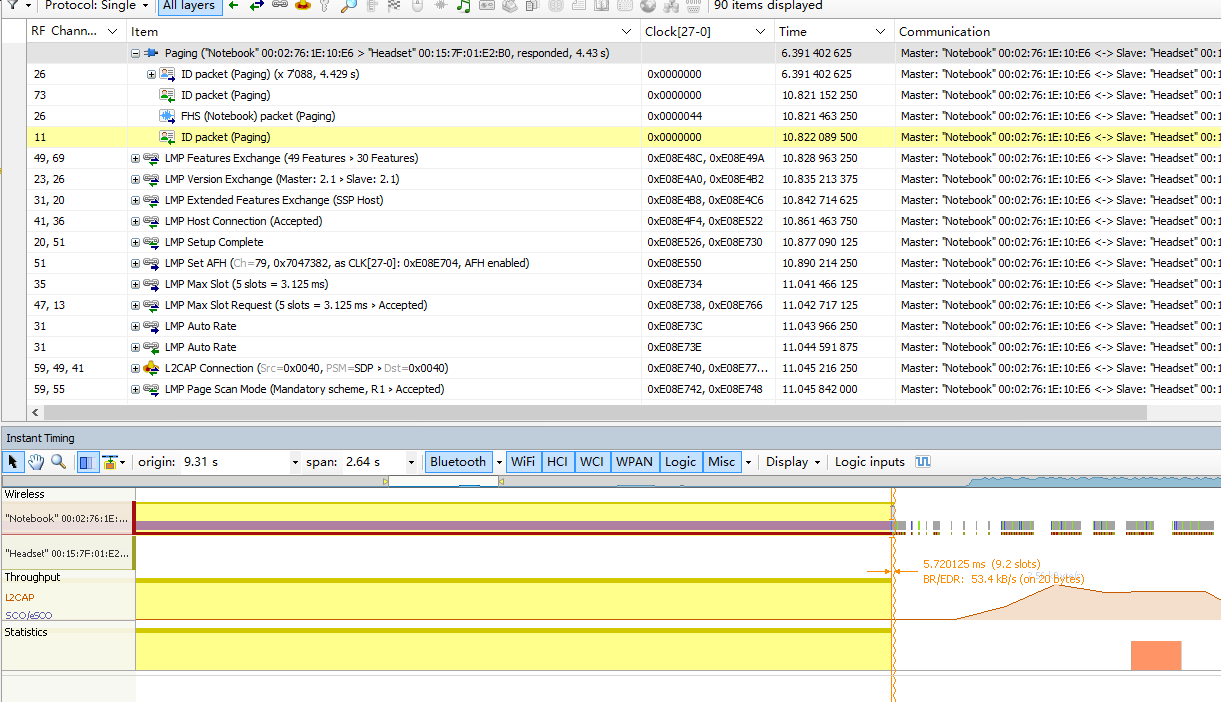
\includegraphics[height=8cm]{page_startup_data.png}
\caption{pagestartupdata}
\label{fig:page_startup_data}
\end{figure}

\href{https://en.wikipedia.org/wiki/Diffie%E2%80%93Hellman_key_exchange}{wiki链接}
\begin{figure}[H]
\centering
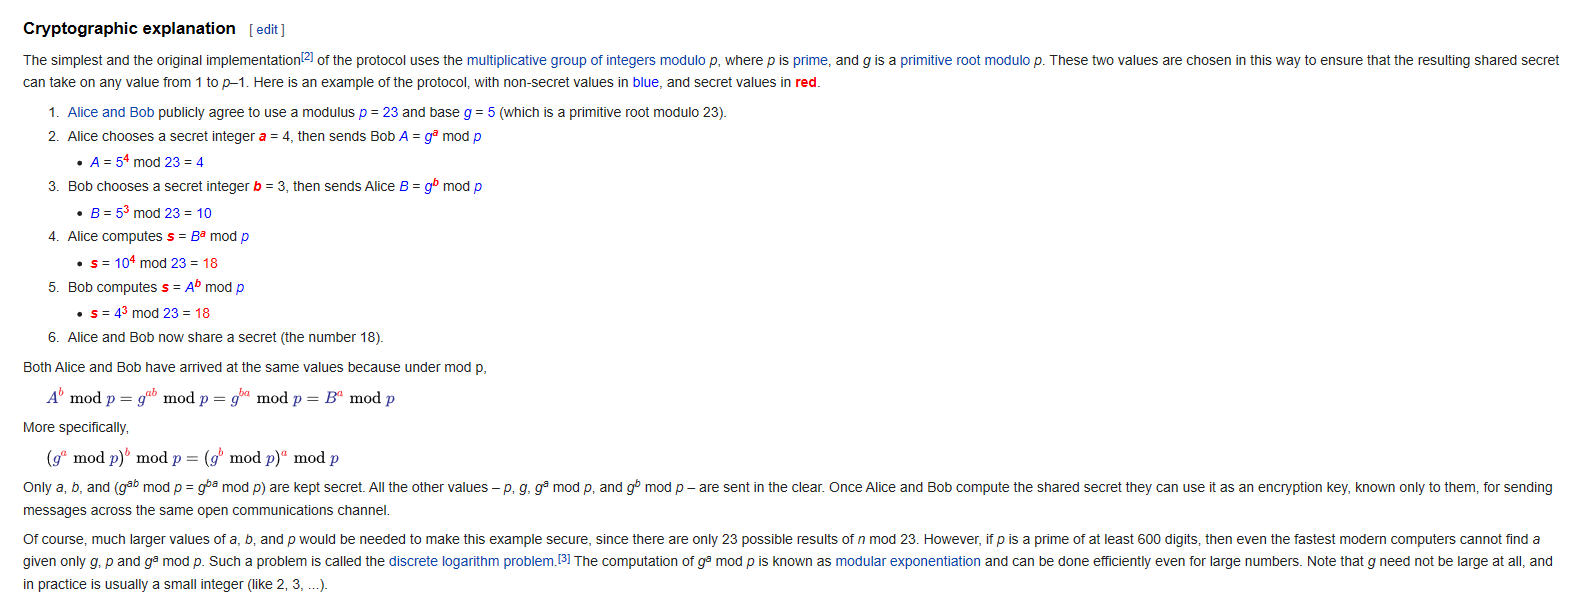
\includegraphics[height=8cm]{wiki1.png}
\caption{wiki1}
\label{fig:wiki1}
\end{figure}

\begin{figure}[H]
\centering
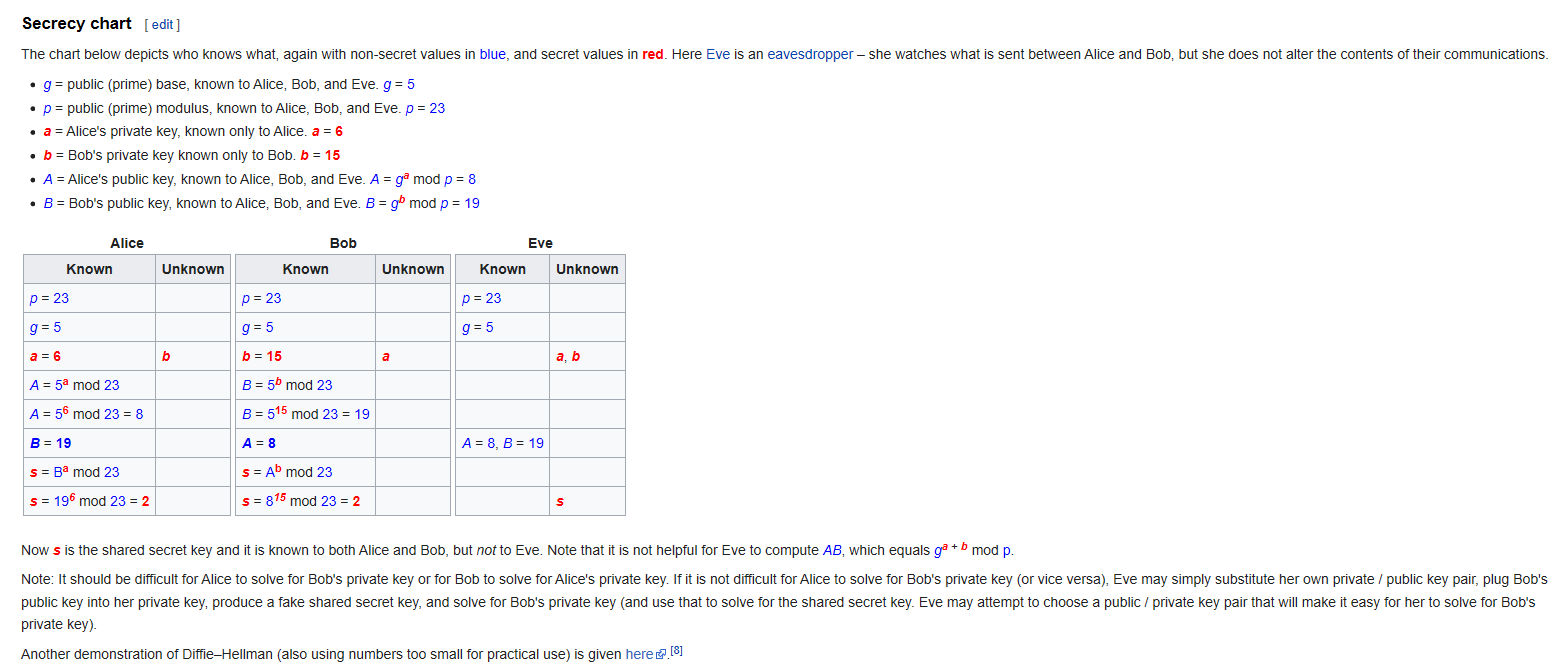
\includegraphics[height=8cm]{wiki2.png}
\caption{wiki2}
\label{fig:wiki2}
\end{figure}

\subsection{USB通信协议}



\section{文学摘抄}
%\begin{itemize}
\subsection{2020年7月28日:《破窑赋》}
%\item 2020年7月28日:《破窑赋》

%\begin{literbox}
    天有不测风云,人有旦夕祸福。蜈蚣百足,行不及蛇;雄鸡两翼,飞不过鸦。马有千里之程,无骑不能自往;人有冲天之志,非运不能自通。

    盖闻:人生在世,富贵不能淫,贫贱不能移。文章盖世,孔子厄于陈邦;武略超群,太公钓于渭水。颜渊命短,殊非凶恶之徒;盗跖年长,岂是善良之辈。尧帝明圣,却生不肖之儿;瞽叟愚顽,反生大孝之子。张良原是布衣,萧何称谓县吏。晏子身无五尺,封作齐国宰相;孔明卧居草庐,能作蜀汉军师。楚霸虽雄,败于乌江自刎;汉王虽弱,竟有万里江山。李广有射虎之威,到老无封;冯唐有乘龙之才,一生不遇。韩信未遇之时,无一日三餐,及至遇行,腰悬三齐玉印,一旦时衰,死于阴人之手。

    有先贫而后富,有老壮而少衰。满腹文章,白发竟然不中;才疏学浅,少年及第登科。深院宫娥,运退反为妓妾;风流妓女,时来配作夫人。

    青春美女,却招愚蠢之夫;俊秀郎君,反配粗丑之妇。蛟龙未遇,潜水于鱼鳖之间;君子失时,拱手于小人之下。衣服虽破,常存仪礼之容;面带忧愁,每抱怀安之量。时遭不遇,只宜安贫守份;心若不欺,必然扬眉吐气。初贫君子,天然骨骼生成;乍富小人,不脱贫寒肌体。

    天不得时,日月无光;地不得时,草木不生;水不得时,风浪不平;人不得时,利运不通。注福注禄,命里已安排定,富贵谁不欲?人若不依根基八字,岂能为卿为相?

    吾昔寓居洛阳,朝求僧餐,暮宿破窑,思衣不可遮其体,思食不可济其饥,上人憎,下人厌,人道我贱,非我不弃也。今居朝堂,官至极品,位置三公,身虽鞠躬于一人之下,而列职于千万人之上,有挞百僚之杖,有斩鄙吝之剑,思衣而有罗锦千箱,思食而有珍馐百味,出则壮士执鞭,入则佳人捧觞,上人宠,下人拥。人道我贵,非我之能也,此乃时也、运也、命也。

    嗟呼!人生在世,富贵不可尽用,贫贱不可自欺,听由天地循环,周而复始焉。
%\end{literbox}

%\end{itemize}

\section{编译器特性笔记}
\subsection{关于versioncheck原理优化代码原理}
Q:编译器代码优化是按照c文件为单位还是以函数为单位,如果以函数为单位,为什么类似于文件系统这些是以version\_check函数调用时,整个c文件的函数都会被调用进来?
\begin{itemize}
\item 函数链接是以\_entry标号作为入口,如果一个函数被显示调用,会把这个函数标号加进来链接,链接是以.o为单位,如果一个函数被显示调用,会把该函数的全部标号拉进来链接(包括结构体),如果一个结构体定义了\emphasizebox{used}属性,该标号会被最终链接进来,导致结构体里的函数指针也会被链接进来,这是使用version\_check选择性链接的原理。

\item libc.a这个库比较特殊,一个函数就是一个.o文件。


\end{itemize}

\subsection{C内联汇编}
参考: \myurlfootnote{https://www.ibiblio.org/gferg/ldp/GCC-Inline-Assembly-HOWTO.html}{GCC-Inline-Assembly-HOWTO}

一般为而言,通过 asm(...) 、 \_\_asm\_\_(...) 、 asm volatile(...) 和 \_\_asm\_\_ volatile(...) 来包含汇编指令模板的字符串形式,如果有额外的约束,通过 : 来分割并指定。
\subsubsection{内联汇编模板}
\begin{myccode}
asm ("汇编模板"
 : /* 输出操作数列表, 可空 */
 : /* 输入操作数列表, 可空 */
 : /* 修改了的寄存器列表, 可空 */
 );

asm ("nop"); // 一条 nop 指令, 没有额外的约束
__asm__ ("nop"); // 同上
 asm volatile ("nop"); // 表示不要随便移动(调度) 这条指令的位置
__asm__ volatile ("nop"); // 同上
\end{myccode}

在一些情况下,在内联汇编中使用了一些指令,这些指令会修改特定的寄存器,这个时候就需要在修改了的寄存器列表里面指明。这是因为内联汇编本身是字符串,并不会被解析,所以编译器内部并不能知道内联汇编的语义(即修改了哪些寄存器、有什么输入输出、做了什么事情以及是否能够被任意移动位置)。所以、我们总是需要通过输出,输入还有修改列表来指定。值得注意的是,为了实现 C 语言的调用协议,一些寄存器被用作了特殊的用途,如使用的栈指针寄存器。

\begin{myccode}
// 下面的做法也是危险的, 因为 r0 被修改了, 但是没有指明
__asm__ volatile ("r0 = 0");
__asm__ volatile ("r0 = 0" : : : "r0"); // ok

//另外一些情况下, 我们可能不希望自己分配寄存器的使用, 可以让编译器分配, 这个是还有需要通过%来指明
u32 reg;
__asm__ volatile ("%0 = rets" : "=r"(reg));
printf("rets的值是 %x", reg);
 // 这个时候表示第0个操作数作为输出, 最终编译器会给%0分配一个寄存器,并替换%0。
\end{myccode}

上述例子中的 "=r"(reg) 表示,对应的内联汇编本体会输出一个结果,并且这个结果应该放置到一个寄存器中,即 "=r" 。而 (reg) 则表示,希望编译器绑定 reg 变量和保存结果的寄存器。这样我们可以而通过访问 reg 获取对应的值。

\subsubsection{多条内联汇编}
一些情况下,会需要写多条连续的内联汇编。这个时候正确的做法是,把这些内联汇编语句用一个 \_\_asm\_\_ 块来表示,而不是分开多个 \_\_asm\_\_ 。例如:
\begin{myccode}
// 定义一个宏, 希望能够清空r1, r0寄存器
// 一个错误的做法:
// 下面的做法有多种错误
// 1. 应该使用一个__asm__块来, 而不是分开多个。 否则它们之间可能会插入其它的指令。
// 2. 内联汇编本体中修改了r1, r0寄存器, 但是没有通过修改列表来说明。
#define MACCLR() __asm__ volatile ("r1 = 0"); __asm__ volatile ("r0 = 0")

// 正确一点的做法:
#define MACCLR() __asm__ volatile( \
"r1 = 0 \n\t" \
"r0 = 0 \n\t" \
: \ // 没有输出
: \ //没有输入
: "r1", "r0" \ // 修改了 r1, r0
);

// 更好一些的做法:
// pi32v2中有一条指令
#define MACCLR() __asm__ volatile ("r1_r0 = 0" : : : "r1", "r0");
\end{myccode}

\subsubsection{寄存器约束}
编译器来分配寄存器的时候,需要指定需要分配的寄存器类型,总结如下:
\begin{figure}[H]
\centering
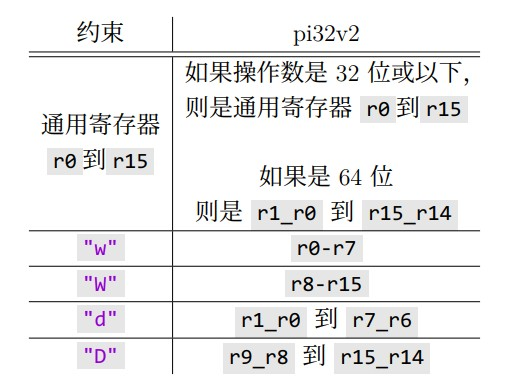
\includegraphics[scale=0.7]{asm_reg.jpg}
\caption{指定分配寄存器}
\label{fig:asm_reg}
\end{figure}
为了方便起见,对于一个 64 位寄存器 DR ,可以用 DR.l 来表示 DR 的低 32 位所在的寄存器, DR.h 用来表示 DR 的高 32 位所在的寄存器。例如r1\_r0.l表示r0,r1\_r0.h表示r1。

\subsubsection{输出约束}
有些时候,我们需要利用内联汇编来获取一些值,这些值需要输出到一些地方,我们通常需要一条输出约束。
\begin{myccode}
unsigned reg;
__asm__ volatile ("%0 = rets" : "=r"(reg));
printf("rets寄存器的值是: %x\n", reg);
// 由上面的汇编说明可以看到, 这个是 pi32v2 的汇编语法
// 表示 %0 表示第一个操作数, 这个是 : 后面开始算起的,
// "=r" 表示这个操作数需要写入到一个寄存器中,
// "=r"(reg) 表示, 输入的寄存器需要和 reg 分配到同一个
// 寄存器, 也就是可以认为把这个结果放入 reg
// 这个指令可以获取当前 rets 的值, 并放入 reg 变量中

__asm__ volatile ("%0 = sp\n" : "=r"(reg));
printf("sp寄存器的值是: %x\n", reg);
// 把 sp 的值存放在 reg 中
__asm__ volatile ("%0 = r4" : "=r"(reg));
printf("r4寄存器的值是 %x\n", reg);
// 获取 r4 的值到 reg 中

__asm__ volatile ("%0 = rets\n" : "=r"(reg));
printf("rets寄存器的值是 %x", reg);
\end{myccode}

\subsubsection{输入约束}
有些时候,我们需要指定一些输入到内联汇编中,这个时候,会需要一条输入约束。
\begin{myccode}
unsigned retaddr = get_retaddr();
__asm__ volatile ("reti = %0\n\t"
"rti \n\t" : : "r"(retaddr));
// "r" 表示这个操作数是被读的, 表示把 retaddr 的值赋值给
// reti, 然后执行 rti 指令, 实现了跳转
\end{myccode}

%值得注意的是,当有多于一条汇编指令需要内联的时候,通常我们写成上述形式,即每行一个汇编指令,并在末尾加上\textbackslash n \textbackslash t,由于内联汇编实际上以字符串形式存储,所以\textbackslash n \textbackslash t 表示换行并插入一个 tab 键。

\subsubsection{earlyclobber 操作数}
编译器在给内联汇编分配寄存器的时候,整块内联汇编被当做一条具有特定输入和输出的指令。并不会关心其内在的含义。例如:
\begin{myccode}
int a, b;
__asm__ volatile (
"%0 = ~ %1\n\t"
: "=r"(a)
: "r"(b));

 //在分配寄存器的过程中, 上面的内联汇编块被当做了
 // <INLINEASM> outs{%0}, ins{%1}
 // 特定于这个例子来说, 如果后续代码不在继续使用 b的值, 而只是使用了a的值
 // 那下面的一些寄存器分配都是合理的
 // 分配方式一:
 // r0 = ~ r0 ; 因为 b 后续不在被使用了, 所以其寄存器可以被a占用
 // 分配方式二:
 // r1 = ~ r0 ; 当然, 也有可能a分配了其它的寄存器
\end{myccode}

另外一些时候,我们的内联汇编块中不会只有一条指令,那么指令之间可能会有先后执行的顺序。这种把所有指令当做一个整体的处理方式,可能会导致问题,例如下面的例子:

\begin{myccode}
int a1, a2;
int b1, b2;
__asm__ volatile (
" %0 = ~ %2\n\t"
" %1 = ~ %3\n\t"
: "=r"(a1), "=r"(a2)
: "r"(b1), "r"(b2)
 );

 // 假设 b2, b1都不在这条指令之后被使用
 // 同样的, 这里在分配寄存器的时候, 还是会被当做下面的东⻄
 // <INLINEASM> outs{%0, %1}, ins{%2, %3}
 // 显然, 如果这个内联块能够作为一条指令整体执行完,
 // 那么下面的一些寄存器分配都是合理的
 // 分配方式一:
 // <INLINEASM> outs{r0, r1}, ins{r0, r1}
 // 即
 // r0 = ~ r0
 // r1 = ~ r1
 // 分配方式二:
 // <INLINEASM> outs{r1, r0}, ins{r0, r1}
 // 即
 // r1 = ~ r0
 // r0 = ~ r1
 // 但是这里, 第二种方式会导致错误的代码
\end{myccode}

上面的例子中,第二种分配方式,如果从一条指令的情况来看,是合理的。毕竟所有的输入一次性使用完毕,然后同时所有的输出被赋值完毕。但是问题在于,输入并不是一次性使用完毕,输出也不是一次性赋值完毕。而是使用一些输入(这里来说,就是第一条 not 指令),然后定义了一些输出,然后又使用了一些输入(这里来说,就是第二条 not 指令),再定义了一些输出。所以,我们需要一个方式标记一些输出,告知编译器这些输出被赋值的时候,还有一些输入没有被使用完,所以,不要让这些输出所使用的寄存器占用输入所使用的寄存器。这种标记方式就是\& 。上面的例子需要修正为

\begin{myccode}
int a1, a2;
int b1, b2;
__asm__ volatile (
" %0 = ~ %2\n\t"
" %1 = ~ %3\n\t"
: "=&r"(a1), "=r"(a2)
: "r"(b1), "r"(b2)
);
// 假设 b2, b1都不再这条指令之后被使用
// & 表示 a1 定义的时候, 输入还没有使用完毕, 也就是说
// 不应该把 a1 定义到 b2, b1 占用的寄存器上
// 对于 a2, 因为 a2 已经是最后一个定义的寄存器, 可以不用加上&
// 因为定义a2的时候, 所有的输入已经使用完毕了
// 当然, 加上也是可以的
\end{myccode}

\subsubsection{输入的同时是输出}
有些操作数是既有读属性,又有写属性的:比如一个后加指令的基地址寄存器,在访问内存后,基地址寄存器的值会被更新,对于这些指令,我们需要两条约束来指定。
\begin{myccode}
void t2sos16(short *in, short *out, int *coeff, int *mem, int npoint, intdstep) 
{
    const int coeffQ = 20;
    const int LeftBit = 8;
    int tmp32_1, tmp32_2, tmp32_3;
    long long tmp64_1;
    asm volatile (
    " %0 += 2<<2 \n\t"
    " %7 = %7 << 1 \n\t"
    "1: \n\t"
    " \n\t"
    " %1 = h[%8++=0] * [%0++=1<<2] (s) \n\t"
    " %4 = %1 >> (%20-%21) (s) # %5 = [%3+0] \n\t"
    " %5 += %4 \n\t"
    " %1 = [%0++=-3<<2] * %4 (s) \n\t"
    " %1 += [%0++=4<<2] * %5 (s) \n\t"
    " %1.l = %1 >>> %20 (up) # %6 = [%3+1<<2] \n\t"
    " %6 += %1.l \n\t"
    " %1 = [%0++=-3<<2] * %4 (s) \n\t"
    " %1 += [%0++=1<<2] * %5 (s) \n\t"
    " %1.l = %1 >>> %20 (up) # [%3+0] = %6 \n\t"
    " %8 += %7 # [%3+1<<2] = %1.l \n\t"
    " %5 >>>= %21 \n\t"
    " %5 = sat16(%5) (s) \n\t"
    " h[%9++=%7] = %5 \n\t"
    " \n\t"
    "if (--%2!=0) goto 1b \n\t"
     : "=&r"(coeff), // 第 0 个操作数, 对应于模板中的 %0
    "=&d"(tmp64_1), // 第 1 个操作数, 对应于模板中的 %1
    "=&w"(npoint), // 第 2 个操作数, 对应于模板中的 %2
    // w 约束了寄存器分配范围, 这是指令要求
    "=&w"(mem), // 第 3 个操作数, 对应于模板中的 %3
    "=&w"(tmp32_1), // 第 4 个操作数, 对应于模板中的 %4
    "=&w"(tmp32_2), // 第 5 个操作数, 对应于模板中的 %5
    "=&w"(tmp32_3), // 第 6 个操作数, 对应于模板中的 %6
    "=&r"(dstep), // 第 7 个操作数, 对应于模板中的 %7
    "=&r"(in), // 第 8 个操作数, 对应于模板中的 %8
    "=&r"(out) // 第 9 个操作数, 对应于模板中的 %9
    : "0"(coeff), // 表示这个操作数需要和 %0 操作数分配到同一个寄存器
    // 这是因为 %0 用作了后加访存指令的基地址操作数, 所以
    // %0 既是一个输入, 也是一个输出
    // "=r"(coeff) 说明了输出, "0"(coeff) 说明同时也是一个输入
    "1"(tmp64_1),
    "2"(npoint),
    "3"(mem),
    "4"(tmp32_1),
    "5"(tmp32_2),
    "6"(tmp32_3),
    "7"(dstep),
    "8"(in),
    "9"(out),
    "i"(coeffQ), // i 表示一个立即数
    "i"(LeftBit)
    :);
}
\end{myccode}

这个例子里面的 coeff 、 tmp64\_1 等,都是既需要读也许要写的操作数。 "=\&r" 表示对应的操作数在指令的输入寄存器使用完成之前就被修改了,这样编译器就不会把输入列表用到的寄存器分配给这些寄存器,这样标记不会导致一些寄存器分配的问题。值得注意的是, "0"(coeff) 之类的约束应该要放置到后面,以防影响操作数顺序。如下面的例子:
\begin{myccode}
int insert(int val_dst, int val_src, int pos, int len)
{
    int pat = (pos << 5) | len;
    __asm__ volatile (
    "%0 <= insert(%1, %2[12:8], %2[4:0])"
    : "=&r"(val_dst),
    : "r"(val_src),
    "r"(pat),
    "0"(val_dst) // 写在最后, 以防影响 %0, %1, %2 顺序
    );

    return val_dst;
}
\end{myccode}

\subsubsection{访问内存}
有时候,我们在内联汇编里面修改了内存,但是由于编译器不知道这个事实,将会导致一些问题。为了解决这个问题,我们需要 "memory" 约束。
\begin{myccode}
// "memory"
int *p = get_ptr();
put_u32hex(*p);
int np = *p + 1;
__asm__ volatile ("[%1] = %0"
: // 没有输出列表
: "r"(np), // 第零个操作数, 对应 %0
// 把 np 的值写入到 *p 的位置
"r"(p) // 第一个操作数, 对应 %1
 : "memory" // 表示内存被修改了
 );
 put_u32hex(*p); // 如果没有上面的 "memory" 可能这个的输出和上一个一样
\end{myccode}

当内联汇编修改了内存的时候,最好加上 "memory" ,这样编译器会失效掉一些缓存了的内存的值。例如上面的 *p ,不过不指定 "memory" 则编译器可能会缓存这个值(为了减少内存访问操作)。

一些例子:
\begin{myccode}
int add(int a, int b)
{
    int c;
    __asm__ volatile (
    "%0 = %1 + %2"
    : "=r"(c) // %0
    : "r"(a), // %1
    "r"(b)); // %2

     // 即 c = a + b
     return c;
}

int add_mem(int *pa, int *pb)
{
    int a, b;
    __asm__ volatile (
    "%0 = [%2] \n\t"
    "%1 = [%3] \n\t"
    "%0 = %0 + %1 \n\t"

    :
    "=&"(a), // %0 输出, 且不能和输入同一个寄存器(⻅earlyclobber操作数)
    "=r"(b) // %1 输出, 可以和输入同一个寄存器
    // (因为定义 %1 的时候, 所有输入都已经使用完毕)
    : "r"(pa), // %2 只是输入
    "r"(pb) // %3 只是输入
);

// 实现了 return *pa + *pb;
return a;
}
\end{myccode}

\section{系统问题总结}
\subsection{关于系统软关机复位问题}
Q:系统软关机使用内置触摸和普通IO关机,开机时\emphasizebox{reset}位置有什么不同?
\begin{itemize}
    \item 普通IO关机,P11系统会掉电,指剩下P33维持电压,开机\emphasizebox{reset}是从\emphasizebox{maskrom}的\emphasizebox{startup}开始;
    \item 使用内置触摸关机,P11系统维持电源工作,这是关机之后还会大几\emphasizebox{uA}的原因,开机\emphasizebox{reset}也是从\emphasizebox{maskrom}的\emphasizebox{Startup}开始;
\end{itemize}

\subsection{关于使用内置触摸开机ROM中IO状态恢复出错问题}
Q:当使用内置触摸开机时,发现\emphasizebox{PC3 IO}变为输出低状态,关机之前在mask\_IO中已经把IO状态设置为高阻?
\begin{itemize}
    \item 当使用\emphasizebox{LPCTMU}关机时,会使用\emphasizebox{PLCNT}模块,配置了\emphasizebox{P3\_PCNT\_SET0}和\emphasizebox{P3\_PCNT\_SET1}两个寄存器,\emphasizebox{PC3 IO}状态正好配置了3,导致在mask恢复IO时设置为输出0状态;
    \item 解决办法:在\emphasizebox{soft\_off\_enter}和\emphasizebox{soft\_off\_exit}时加入\emphasizebox{save}和\emphasizebox{recover}流程即可。
\end{itemize}

\subsection{br28 ass ASS\_CLK\_CON bit7写完和读出来不一样问题(bit5)}
问题:在写ASS\_CLK\_CON的bit7置1时,写完读出来是0x40,再写bit7置0时,读出来时0x20;

解释:由于bit5没有用到,cpu读会移位,在软件层面第一次写bit7置1时,cpu行为:
\begin{myccode}[caption={bit7置1 cpu行为}]
    {
        int bak = 0;
        bak = ASS_CLK_CON;
        bak |= BIT(7);
        ASS_CLK_CON = bak;
    }
\end{myccode}
由于bit5没用到,在cpu读时,bit6变bit5,bit7变bit6,因此写完bit7之后,读出来是0b0100,0000 = 0x40,再把bit7写0时,cpu行为:
\begin{myccode}[caption={bit7置0 cpu行为}]
    {
        int bak = 0;
        bak = ASS_CLK_CON;  //此时bak = 0b0100,0000
        bak &= ~BIT(7);     //此时bak = 0b0100,0000
        ASS_CLK_CON = bak;  //写bit7为0无效;
    }
\end{myccode}
下次再写bit7,将会读回来是0b1100, 0000 = 0xC0,导致出错,硬件Bug;

\subsection{br34 RVDD电压要大于等于DVDD问题}
如果RVDD < DVDD时,有的板子会出现程序跑到某个ram地址出现非对齐访问异常问题。
\begin{figure}[H]
\centering
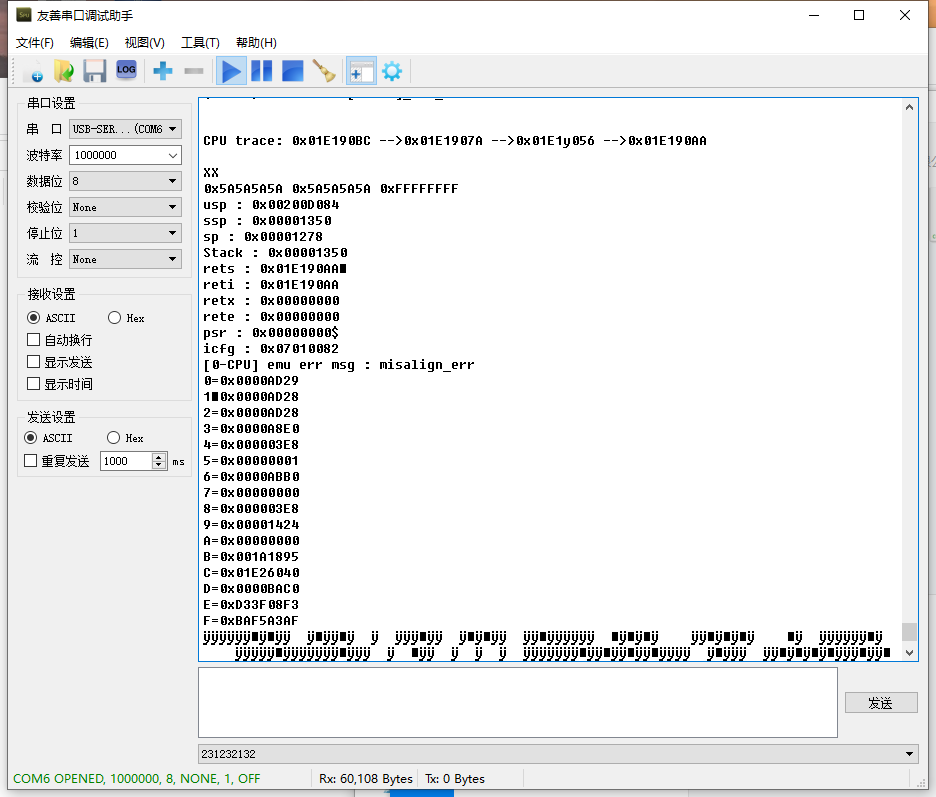
\includegraphics[height=8cm]{rvdd_question.png}
\caption{异常打印}
\label{fig:rvdd_exeception}
\end{figure}
注意:RVDD >= DVDD。


\subsection{有符号数十六进制转十进制计算方法}
计算机内存数值存储方式
1)原码:一个数的原码(原始的二进制码)有如下特点:
\begin{itemize}
\item 最高位做为符号位,0表示正,1表示负
\item 其它数值部分就是数值本身绝对值的二进制数
\item 负数的原码是在其绝对值的基础上,最高位变为1
\item 原码表示法简单易懂,与带符号数本身转换方便,只要符号还原即可,但当两个正数相减或不同符号数相加时,必须比较两个数哪个绝对值大,才能决定谁减谁,才能确定结果是正还是负,所以原码不便于加减运算
\end{itemize}

2)反码
\begin{itemize}
\item 对于正数,反码与原码相同
\item 对于负数,符号位不变,其它部分取反(1变0,0变1)
\item 反码运算也不方便,通常用来作为求补码的中间过渡
\end{itemize}

3)补码
\begin{itemize}
\item 对于正数,原码、反码、补码相同
\item 对于负数,其补码为它的反码加1
\item 补码符号位不动,其它位求反,最后整个数加1,得到原码
\item 在计算机系统中,数值一律用补码来存储
\end{itemize}

4)计算机系统中,数值一律用补码来存储,主要原因是:
\begin{itemize}
\item 统一了零的编码,0在计算机中存储的方式:
\begin{myccode}[caption=zero 编码]
        int a = 0; int b = -0;
        0000 0000     1000 0000
\end{myccode}
\item 为了统一0的编码,计算机中没有-0的概念
\item 将符号位和其它位统一处理,在数据计算中,符号位也参与程序的计算
\item 将减法运算转变为加法运算,计算机只会算加法10+(-10)
\item 两个用补码表示的数相加时,如果最高位(符号位)有进位,则进位被舍弃
\end{itemize}

5)将一个十六进制的有符号数转换为十进制数实例:
\begin{itemize}
\item 十六进制数:0xFFF4 = 0b1111,1111,1111,0100
\item 除了符号位求反码: = 0b1000,0000,0000,1011
\item 原码 = 反码+1:    = 0b1000,0000,0000,1100
\item 原码十进制 = -12
\end{itemize}


\section{软件安装总结}
\subsection{GVIM安装}
\begin{itemize}
\item GVIM安装包链接:\url{https://pan.baidu.com/s/1PcF6-taEaOIg66kbnm6EPA},提取码:66u3。
\item 解压压缩包到任意目录。
\item 运行\emphasizebox{install.exe}
\begin{messagebox}
This program sets up the installation of Vim 8.1

Inspecting system...


Install will do for you:
 1  Install .bat files to use Vim at the command line:
 2      Create C:\WINDOWS\vim.bat
 3      Create C:\WINDOWS\gvim.bat
 4      Create C:\WINDOWS\evim.bat
 5      Create C:\WINDOWS\view.bat
 6      Create C:\WINDOWS\gview.bat
 7      Create C:\WINDOWS\vimdiff.bat
 8      Create C:\WINDOWS\gvimdiff.bat
 9      Create C:\WINDOWS\vimtutor.bat
10  Do NOT change startup file D:\Vim_8_1\_vimrc
14  Install an entry for Vim in the popup menu for the right
    mouse button so that you can edit any file with Vim
15  Add Vim to the "Open With..." list in the popup menu for the right
    mouse button so that you can edit any file with Vim
16  Add Vim to the Start menu
17  Create a desktop icon for gVim
18  Create a desktop icon for gVim Easy
19  Create a desktop icon for gVim Read-only
20  Do NOT create plugin directories
To change an item, enter its number

Enter item number, h (help), d (do it) or q (quit):
\end{messagebox}
\item 选项14是在文件夹空白地方右击弹出vim,不需要点文件;
\item 选项15是在文件夹里的文件右击弹出vim;
\item 实际选择15即可;
\item 注意输入方法, 先输入15,回车\emphasizebox{Enter}
\item 再输入d(do), 回车\emphasizebox{Enter}
\item 添加全局变量,在系统变量添加路径;
\begin{messagebox}
D:\Vim_8_1\vimfiles\tools
\end{messagebox}
\item 直接右击文件用vim打开即可,但还存在字体兼容问题;
\item 安装字体,文件路径
\begin{messagebox}
D:\Vim_8_1\vimfiles\fonts\airline\UbuntuMono
\end{messagebox}
\item 可使用\emphasizebox{RightMenuMgr}工具增加右击打开\emphasizebox{GVIM}
\end{itemize}



\end{document}


